\section{Experiments} \label{sec:experiments}

Due to the difficulty in finding publicly available audio odometry datasets,
the problem of robot localization is simplified to a single dimension over a
unique terrain type: A wheel that can only move along a longitudinal axis over
loose sandy terrain. As this scenario can be easily reproduced with the
available \nameref{subsec:experimental-setup}, making it possible
to gather a whole new \nameref{subsec:datasets}. Experiments are conducted
varying the different tuneable parameters in the
\nameref{subsec:feature-extraction} module and \nameref{sec:prediction-model}
and a model is selected based on its performance and computational cost.

\include*{\subdir/experimental-setup}

\subsection{Datasets} \label{subsec:datasets}

\subsubsection{Training}
used to train and validate the \nameref{sec:prediction-model}. This work
defines it as a collection of annotated overlapping segments.

The annotated variables are the longitudinal velocity $V_x$, the wheel angular
speed $V_\omega$ and the slip ratio $s$. However, as it has been explained in
\cref{sec:prediction-model}, these segments are relatively large in terms of
time. In a way that the measured variables can oscillate significantly during
the segment. This work annotates the segments with a weighted average of the
measurements within its duration.

% Consider $x[t]$ the measurement of a given variable $x$ at time $t$, being $t$
% in the set of measurement times $t \in T$. \Cref{eq:segment-labeling} describes
% how the weighted average of that variable $x$ is computed for segment $k$ where
% $t_k$ is the vector of measurement times inside the segment boundaries and $N$
% its size. 

% \begin{equation}
%     x_k = \frac{\sum_{i = 1}^N i  x[t_k[i]]}{\sum_{i = 1}^N i}\text{, where } i \in  \mathbb{N}
%     \label{eq:segment-labeling}
% \end{equation}

Segments are collected from a set of training recordings captured under
different driving conditions, which are defined by the combination of the
following controlled variables: \emph{slip ratio} as defined in
\cref{eq:slip-ratio}. Ranging between -0.3 and 0.6. Being free or uncontrolled
slip an additional option; \emph{load} measured in kg added to the base
carriage weight (which is 11.2 kg) taking values of 0 kg, 5 kg and 10 kg;
\emph{wheel angular velocity} ranging from 5 deg/s to 30 deg/s in steps of 5
deg/s; \emph{contact}, whether the wheel is making contact with the ground or
is suspended in the air. A total of 168 different recordings that make a total
of 1 hour for each of the 8 recording devices where captured for the training
dataset.

% One can visualize in \cref{fig:datasets-segments} the segments with their
% longitudinal velocity $V_x$ annotations computed from the measurements that lay
% inside the segment boundaries as described by \cref{eq:segment-labeling}.
% Moreover, \cref{fig:dataset-visualization} shows consecutive segments from one
% of the datasets used in this work with their complete annotations.
% \Cref{fig:dataset-visualization} also shows the distribution of the values of
% the variables of interest in the dataset. This distribution can be altered
% employing \nameref{subsec:data-augmentation} and \nameref{subsec:data-split} in
% order to obtain a more favorable distribution for model training.

% \begin{figure}
%     \centering
%     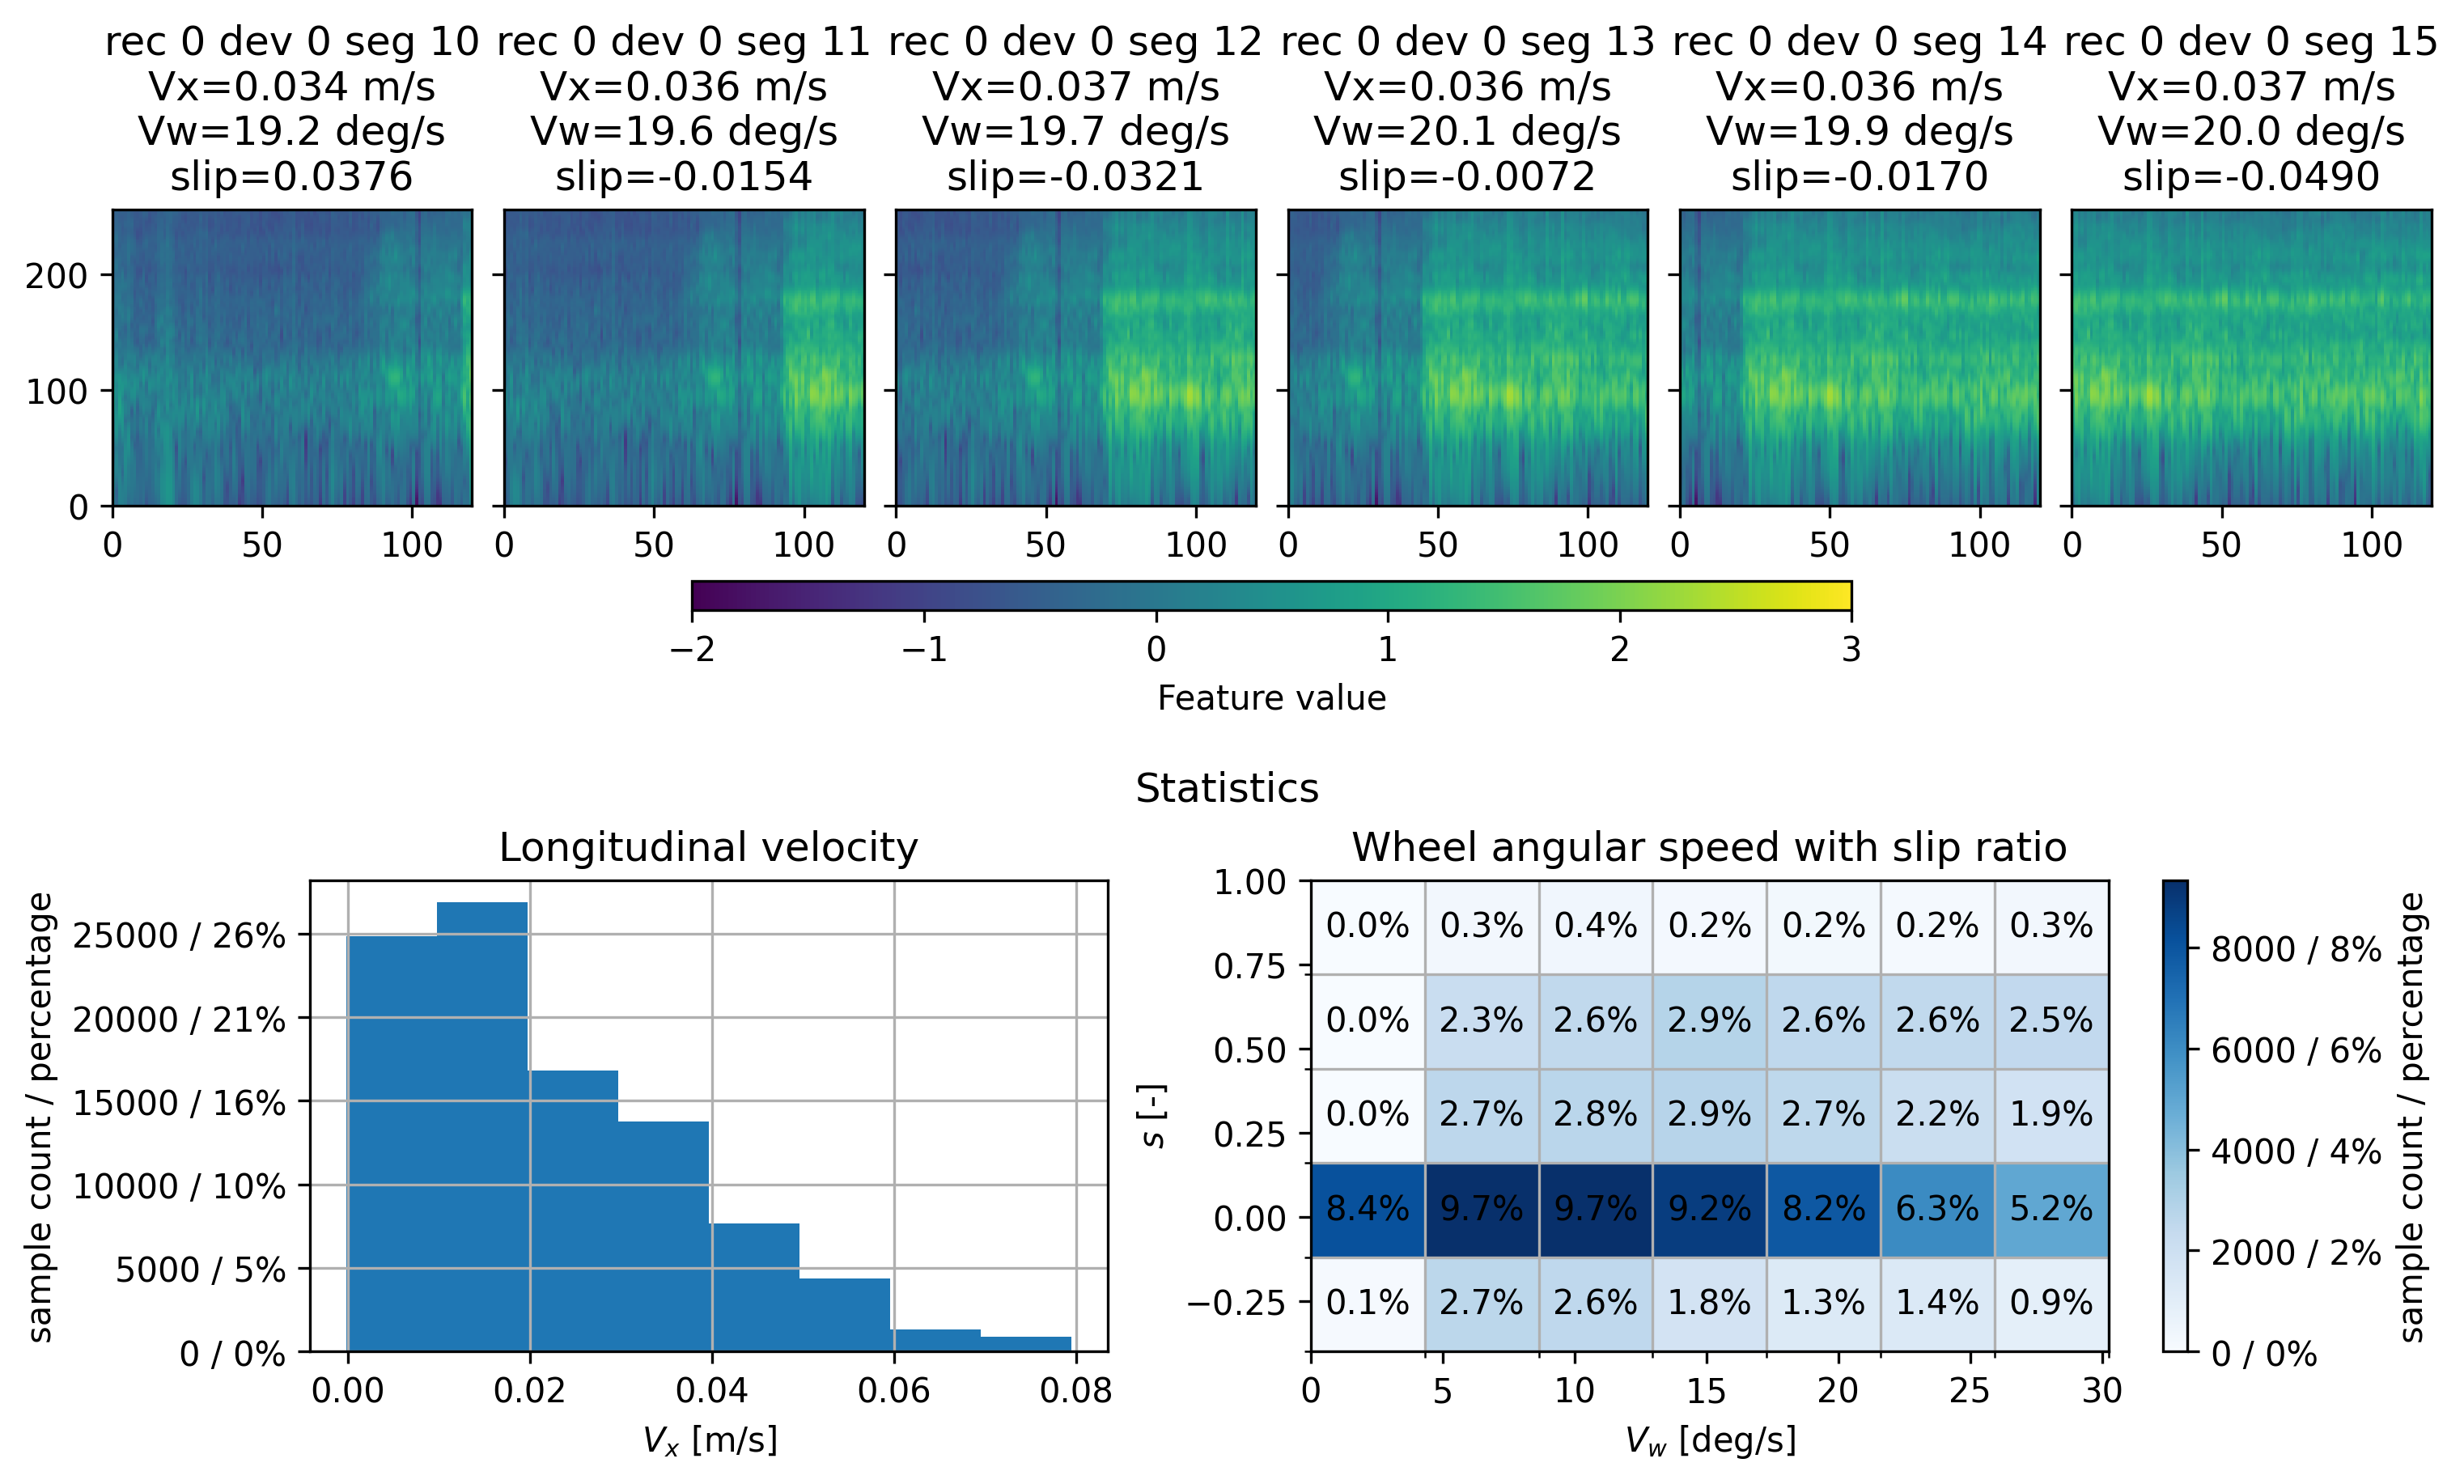
\includegraphics[width=\linewidth]{\subdir/dataset.png}
%     \caption[Dataset visualization]{Visualization of consecutive samples from a
%         dataset together with the distribution of the variables of interest.
%         This dataset was processed using all available recordings from
%         \nameref{subsec:wheel-testbed-experiment-2}, a single
%         \nameref{subsubsec:gammatone-filterbank} extractor with 256 features
%         per frame, a frame duration of 10 ms and a segment length of 100 frames
%         with 80\% overlapped frames between consecutive segments. }
%     \label{fig:dataset-visualization}
% \end{figure}

The collected segments are artificially augmented using two methods: Add a
random gain in the range [-10, 10]; Add white noise with a random
signal-to-noise ratio in the range [0, 1] in the decibel scale.

\subsubsection{Evaluation}
used to evaluate the performance of the system under more realistic and
challenging conditions unseen during training. 

\subsection{Selected model} \label{sec:selected-model} 

This work selects a model trained on a dataset of segments of 50 frames, each
of them spans over 15 ms and has 64 features from a single
\nameref{subsubsec:gammatone-filterbank} extractor. The extractor is applied on
the average of the audio signal channels with a frequency range of [50, 80000]
Hz and features on te Bel scale. Training data from all available recordings is
selected using the \texttt{with-laptop} strategy split described in
\cref{table:training-data-split}, a \nameref{para:model-task-ord-class} task
with 28 different linearly distributed longitudinal velocity ranges and a
\nameref{para:model-arch-norm-cnn} architecture with a small size described as
\texttt{S} in \cref{table:model-arch-sizes}. 